\chapter[Texas Instruments TMS320C6678]{Texas Instruments\\TMS320C6678}
\label{chapter:c6678}
This chapter describes the Texas Instruments TMS320C6678 multicore DSP. First
the selection of the TMS320C6678 as the hardware platform for the experiments
is explained. Second an overview of the hardware platform and the associated
development tools is presented. Third the key hardware features of the 
platform are examined.

\section{Motivation}
The hardware platform used in the experiments in this thesis is the  
Advantech TMDSEVM6678L TMS320C6678 Evaluation Module. The processor in the
evaluation module is the Texas Instruments TMS320C6678. The TMS320C6678
is a fixed and floating point digital signal processor based on the
Texas Instruments Keystone I architecture. The processor has eight
C66x DSP cores at 1.0 GHz clock frequency \cite{tmsdatasheet}.

The TMS320C6678 was chosen as the hardware platform for the experiments
for two main reasons. First the Keystone I architecture is designed with
stream processing applications in mind \cite{multicorevideo}. Second the
objective of this thesis is to understand hardware and software features
supported by the TMS320C6678.

The specific features in the TMS320C6678 we are interested in are the
support for OpenEM included in the MCSDK for Keystone I devices
\cite{MCSDKbrochure} and the hardware accelerated scheduling and
communication utilized by the OpenEM runtime. 

An additional benefit of choosing TMS320C6678 as the hardware platform for
the experiments is the support for the platform in PREESM
\cite{pelcat2014preesm}.
\section{Overview}

\begin{figure}[h!]
    \label{arch_overview}
    \begin{center}
        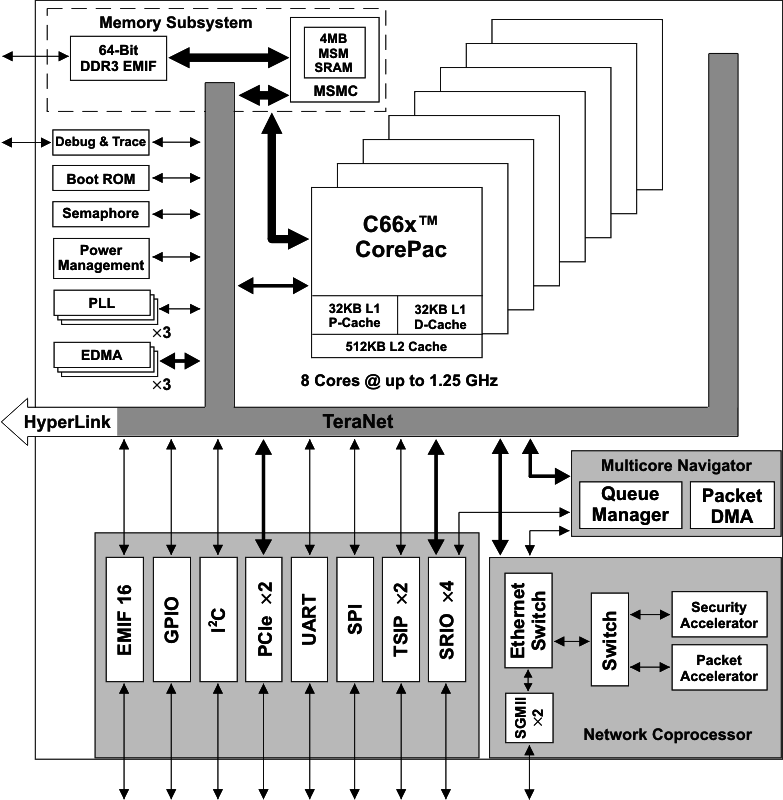
\includegraphics[width=0.99\textwidth]{fbd_SPRS691e.png} % Include the image placeholder.png
        \caption{Overview of the TMS320C6678 architecture.}
    \end{center}
\end{figure}

Keystone I architecture
Explain the evaluation module
Development tools

\section{Hardware Features}
\subsection{C6678 Cores}
Pipeline
Vector instructions
\subsection{Memory}
Caches
MSMC
Off chip memory in the EVM
\subsection{Multicore Navigator}
QMSS
PDSP


